\section{Process Perspective}

\subsection{Organization of the Team}
We have primarily met on Tuesdays at ITU before the lecture to work on the project together. We usually stay throughout the exercise session to do the exercises and some project work. At the end of the session, we usually distribute the task that should be worked on. For communication, we have used Facebook Messenger for quick day to day coordination, and a Discord server for knowledge sharing, planning, and discussions.
We've used GitHub projects as a kanban board for the tasks that needs to be done, but slowly drifted away from using this towards the end of the project, mostly because the amount of tasks got more manageable to the team size. 


\subsection{Organization of your repository}
The whole system is stored in a mono repository on Github. We never found a reason to split our repository up. We did not reach a size of the codebase, where we lost track of the structure, and our layered architecture did not make much sense to split up into multiple repositories.


\subsection{Branching strategy}
During this project, to avoid risking downtime during deployment, we used the GitLab Flow branching strategy. However, after implementing Docker swarm with rolling updates, we've been less concerned with downtime. For this reason, had we continued work on this project for
longer and given our team size, we would have used Trunk-Based branching strategy. We think having small lived branches that get merged frequently to the mainline is the most effective way to incrementally and quickly deploy new features, which is the whole point of DevOps.


\subsection{CI/CD}

\begin{figure}[H]
    \centering
    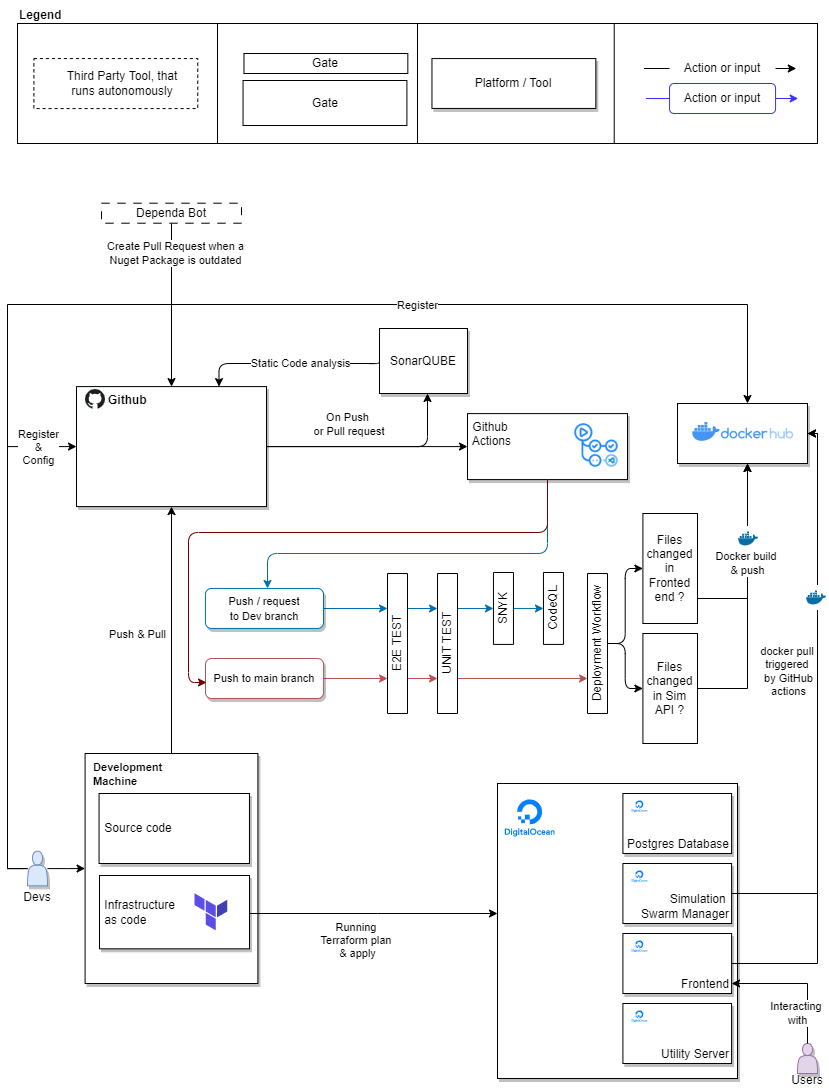
\includegraphics[width=\linewidth]{images/Pipeline.png}
    \caption{Our current pipeline as of finishing the project}
    \label{fig:ci_cd_pipeline}
\end{figure}

Our CI/CD relies heavily on GitHub Actions, and we actually ended with a pipeline similar to our planned pipeline.\ref{fig:CICD}
\subsubsection{Continuous deployment} 
It happens when a push has been made to the main branch, which upon agreement (meaning no enforced restrictions on GitHub) happens when we successfully push to the main branch, usually by creating a release.
\\
When a successful push has been made, we run our test suite, which acts as a gate for the following steps. Because we are using a mono repository, we then check whether a change has occurred in the frontend folder or in the backend folder and build and push the docker images to docker hub accordingly. This led to us having two different docker images for the frontend and for the simulation API, respectively. If an image is successfully build and pushed, we then use a workflow to ssh into the correct machine and do a docker pull. 
The idea behind this workflow was that we didn't like that changes to the frontend killed the API server and vice versa, and ultimately meant that we split the API and frontend into two different services hosted on different servers.
\subsubsection{Continuous integration}
It happens whenever a push or a pull request occurs on the development branch. 
Just like our CD workflow it runs our unit test suite, and you could argue that it makes the testing suite in the deployment workflow redundant, but given that we didn't have any enforced rules on pushing to the main branch, we felt that it was best to keep it there as a safety. We also don't run the E2E test in this workflow, as the E2E in playwright didn't work nicely with GitHub Actions, but would have worked similar to the gate for the docker build \& push in the CD where it would only run on changes in the frontend folder.
It then runs linting for our docker files as well as image security using Snyk.
We then perform code security analysis on our CSharp code using CodeQL. We also use SonarQube on a pull request to check for code smells, vulnerabilities, security Hotspots, Code smells. Our CI/CD might seem disconnected from each other in our current workflow and this is a product of our current branching strategy. When we eventually would have made the switch to trunk based branching, we would have liked to combine the two as a single workflow. This workflow would run on changes on the main branch as we believe that CI is a step to reach CD, and it therefore doesn't make sense to have them as separated as we currently do.

\subsection{Development process and tools}
We organized our work with a Github Project which allowed us to easily keep track of issues and their progress. Dragging these issues around in a Kanban board gave a nice overview of what needed to be worked on. We also used some automation that would add issues on GitHub to the kanban board automatically.

\subsection{Monitoring}

\subsubsection{NetData}
NetData helps us monitor the performance and health of the hardware of our system's nodes, however the usefulness of NetData got diminished when we switched our simulation API to be distributed through docker swarm as we only received performance metrics for the current main worker.

\subsubsection{Prometheus}
We used Prometheus to monitor our application's performance, collect metrics from various components and gain insights into the health and behavior of our infrastructure.
We collect service specific metrics from our simulation API like number of registered users and the amount of twits sent. 

\subsubsection{Visualization}
Grafana has allowed us to take the data collected from Prometheus, and visualize it in a dashboard.

\subsection{Logging}
We log all the request being made by our users, and sort the logs by assigning them levels such as Information for when things go as planned, Error when there occurs an error and Fatal it there occurs a critical error. We use Serilog, a Nuget package, as an alternative to Logstash, for sending logs to Kibana.

\subsection{
Brief results of the security assessment.}
Using a Kali Linux Docker container as described in the Security Exercise\footnote{\url{https://github.com/itu-devops/lecture_notes/blob/master/sessions/session_09/README_EXERCISE.md}}, we scanned our site with WMAP in Metasploit, which yielded no warnings for our system at the time. 
\subsection{Strategy for scaling and load balancing}
The Docker Swarm manager balances requests for our simulation within the cluster.\cite{dockerswarm} We still have to manually change our docker compose to do more replications but would have loved to have some kind of system in place to do this automatically like Kubernetes. We could easily have expanded to use docker Swarm  to the frontend and if need be the utility server, but felt like this was unnecessary.




\subsection{AI-assistants}
\subsubsection{Explain which system(s) you used during the project.}
We have used ChatGPT lightly as an alternative to asking a TA and mostly for trivial questions as it has a tendency to lie when asked non-trivial questions.
We have also used for generating skeleton files for things like docker-compose etc. this works fine, but you need to know what it is doing as it is very capable of making mistakes.
\subsubsection{Reflect how it supported/hindered your process.}
I would say it aided in our process. It is great at giving more precise information whenever a tools' documentation is lackluster, it also is good at writing boilerplate code / configs, but you have to review the output as it is often faulty, outdated, or straight up wrong.